\documentclass[11pt,a4paper]{article}
\usepackage[margin=24mm]{geometry}
\usepackage[T1]{fontenc}\usepackage[utf8]{inputenc}\usepackage{lmodern}\usepackage{microtype}
\usepackage{amsmath,amssymb,bm}\usepackage{booktabs,tabularx,longtable,array}
\usepackage{graphicx}\usepackage[dvipsnames]{xcolor}
\usepackage{hyperref}
\usepackage{fancyhdr}\usepackage[numbers,sort&compress]{natbib}
\definecolor{reportblue}{HTML}{174A7E}\definecolor{reportgreen}{HTML}{2E7D32}\definecolor{reportorange}{HTML}{C76B00}\definecolor{reportred}{HTML}{A52521}\definecolor{reportgray}{HTML}{F3F5F7}
\hypersetup{colorlinks=true,linkcolor=reportblue,citecolor=reportblue,urlcolor=reportblue,pdftitle={Structured SO(3) Latents with Physics-Residual Artifacts}}
\setlength{\parindent}{0pt}\setlength{\parskip}{.55em}
\setlength{\headheight}{14pt}
\pagestyle{fancy}\fancyhf{}\lhead{Structured $SO(3)$ Latents and Residual Artifacts}\rhead{21 September 2026}\cfoot{\thepage}
\newcommand{\R}{\mathbb R}\newcommand{\SO}{\mathrm{SO}}\newcommand{\so}{\mathfrak{so}}\newcommand{\Exp}{\operatorname{Exp}}\newcommand{\sg}{\operatorname{sg}}\newcommand{\vct}[1]{\bm{#1}}
\newenvironment{keyresult}{\begin{quote}\color{reportgreen}\textbf{Key result.} }{\end{quote}}
\newenvironment{caution}{\begin{quote}\color{reportorange}\textbf{Important qualification.} }{\end{quote}}
\newenvironment{verdict}{\begin{quote}\color{reportblue}\textbf{Research verdict.} }{\end{quote}}
\begin{document}
\begin{titlepage}\centering\vspace*{22mm}
{\Huge\bfseries\color{reportblue} Ball World Model\par}\vspace{5mm}
{\LARGE Structured $SO(3)$ and $\so(3)$ Latents with Physics-Residual Artifact Disentanglement\par}\vspace{15mm}
\fbox{\parbox{.87\textwidth}{\centering\large A detailed architectural, mathematical, and empirical analysis of a rotation-only visual observer}}
\vfill{\Large Dr. Jasper Juchem\par}\vspace{5mm}
{\large Stand-alone technical report for AI, machine-learning, world-model, and dynamical-systems researchers\par}\vspace{12mm}
{\large Evaluation dated 21 September 2026\par}{\large Version 1.0\par}
\end{titlepage}

\begin{abstract}
This report studies a visual observer for a textured rigid sphere undergoing rotation with fixed centre and constant world-frame angular velocity. The observer is designed around a structured latent representation rather than a generic Euclidean vector. Its context latent contains a canonical $SO(3)$ group element, a high-dimensional $K=24$ equivariant carrier, scalar invariant features, and observation artifacts. Its motion latent contains a canonical $\so(3)$ generator, the induced carrier tangent, scalar motion features, and a motion-artifact sector. The intrinsic rotational transition is $G_{t+1}=\Exp(\Delta t[\xi_t]_\times)G_t$. Decoded-state refinement is disabled, so rotational geometry is introduced in the latent itself.

The previous structured model showed that the designated group and algebra sectors were valid and operational, but a held-out probe recovered angular velocity from motion artifacts with mean component $R^2\approx0.997$. The new model therefore changes artifact learning. A physics-conditioned network first predicts the feature-map rate explained by $(F_t,G_t,\xi_t,\Delta t)$. The artifact encoder receives only the stopped-gradient residual. A residual decoder gives the artifact sector a positive reconstruction task, while gradient-reversal adversaries and cross-covariance regularisation discourage angular velocity and relative rotation from remaining in the artifact representation.

The new model preserves strong physical accuracy. Mean orientation error is $0.566^\circ$ and angular-velocity $R^2$ remains between 0.9974 and 0.9991. Generator accuracy improves on every axis relative to the previous structured model, while orientation accuracy becomes worse. Intrinsic one-step transition error remains nearly unchanged, and nine-interval rollout has slightly higher mean error but lower 95th-percentile error. The zero-artifact bypass test gives exactly zero angular-velocity change, confirming that the physical output does not causally depend on the post-split artifact vector.

The disentanglement goal is only partly achieved. Artifact-to-angular-velocity mean $R^2$ decreases from approximately 0.9969 to 0.9926, which is measurable but small; artifacts still contain almost all signed rotational motion. The scalar motion sector improves much more, falling from mean $R^2\approx0.886$ to $0.281$. The results therefore support a precise conclusion: residual and adversarial training improves the allocation of some auxiliary sectors and preserves the structured physical pathway, but it does not yet isolate the artifact latent from rotational information. The report explains why this outcome is plausible and identifies the architectural and data-level changes needed for stronger separation.
\end{abstract}
\tableofcontents\clearpage

\section{Problem formulation and experimental scope}
\subsection{Physical system}
The observed object is a rigid sphere with fixed centre. Translation is suppressed, so position and linear velocity are constant and excluded from the present model. The varying physical state is
\begin{equation}
(R_t,\omega_t)\in SO(3)\times\so(3),
\end{equation}
where $R_t$ maps body-frame vectors into the world frame and $\omega_t\in\R^3$ is the world-frame angular velocity. For a sampling interval $\Delta t$, ideal constant-angular-velocity motion satisfies
\begin{equation}
R_{t+1}=\Exp(\Delta t[\omega_t]_\times)R_t.
\end{equation}
The cross-product matrix $[\omega]_\times$ is skew symmetric, hence an element of $\so(3)$. Its exponential is a proper rotation.

The input is a context of ten rendered RGB images,
\begin{equation}
I_{1:T}\in\R^{B\times T\times3\times256\times256},\qquad T=10.
\end{equation}
Four coloured surface markers break the rotational symmetry of an otherwise spherical body. Ground-truth orientation and angular velocity are available during supervised training but not as inputs at inference.

\subsection{Why a Euclidean latent is not sufficient for the research question}
A generic latent transition
\begin{equation}
z_{t+1}=z_t+\Delta t f_\theta(z_t,m_t),\qquad z_t\in\R^d,
\end{equation}
can approximate one-step observations, but it does not encode the noncommutative composition law of three-dimensional rotations. A decoder can map $z_t$ onto a valid rotation after the fact, yet the internal transition remains an additive operation. The objective of this project is stronger: a designated latent sector should itself support group multiplication, inversion, and Lie-algebra-generated motion.

\subsection{Why artifacts require a separate treatment}
Images contain more than physical state. Lighting, shadows, antialiasing, visibility, marker appearance, background, camera motion, and sensor effects can change observations without changing the physical configuration in the same way. A useful observer should preserve such information when needed without allowing it to replace the physical state. The desired decomposition is therefore
\begin{equation}
\text{observation information}=\text{structured physical information}+\text{observation residual}.
\end{equation}
The central challenge is identifiability. If the same visual variation is statistically correlated with rotation throughout the dataset, an unconstrained artifact branch has no reason not to copy rotation.

\section{Structured context latent}
\subsection{Coordinate-aware spatial encoder}
Each RGB frame is augmented by normalized horizontal and vertical coordinates. A shared convolutional backbone produces a spatial feature map
\begin{equation}
F_t\in\R^{128\times16\times16}.
\end{equation}
Keeping a spatial map is important because rotational cue fields are local: different markers move in different directions and can be visible or occluded at different locations. Global pooling before differencing could destroy this information.

A soft-keypoint readout produces coordinates, variances, confidence terms, and locally weighted appearance vectors. These statistics are projected to a frame descriptor $d_t\in\R^{256}$.

\subsection{Canonical group sector}
The descriptor predicts six unconstrained coordinates. These are mapped continuously to a rotation matrix using the first-two-column construction and Gram-Schmidt orthogonalisation. Continuous 5D and 6D representations avoid discontinuities that affect lower-dimensional Euclidean rotation parametrisations \citep{zhou2019rotation}. The resulting matrix satisfies
\begin{equation}
G_t^TG_t=I,\qquad\det G_t=1.
\end{equation}
This matrix is not merely a decoder output. It is the canonical rotational context variable used by the latent transition.

\subsection{High-dimensional equivariant carrier}
A three-dimensional manifold need not use only three ambient coordinates. To preserve representational richness, the model contains 24 body-frame template vectors $b_k\in S^2$. The first four correspond to marker directions; the remaining templates provide broader directional coverage. The visual encoder predicts a non-negative scalar amplitude $\alpha_{t,k}$ for each channel and constructs
\begin{equation}
u_{t,k}=\alpha_{t,k}G_tb_k.
\end{equation}
Under a change of world-frame basis $Q\in SO(3)$,
\begin{equation}
u_{t,k}\mapsto Qu_{t,k}.
\end{equation}
The carrier is therefore equivariant by construction. Its 72 coordinates form 24 copies of the standard vector representation. The amplitudes can represent cue strength, confidence, or visibility while the vector directions retain a prescribed group action.

\subsection{Scalar and context-artifact sectors}
The context latent also contains 16 scalar coordinates $c_t$. Scalar means invariant under the group action, not constant in time. These coordinates can represent confidence or observability without rotating like vectors. A 138-dimensional context-artifact sector $a_t$ is unrestricted and intended for appearance information not needed by physical dynamics.

The packed context has dimensions
\begin{center}\begin{tabular}{lrr}\toprule
Sector & Dimension & Geometric type\\\midrule
Continuous rotation chart & 6 & parameterises $SO(3)$\\
Carrier amplitudes & 24 & scalars\\
Carrier vectors & 72 & vector representation\\
Physical scalar sector & 16 & trivial representation\\
Context artifacts & 138 & unrestricted\\\midrule
Total & 256 & mixed\\\bottomrule
\end{tabular}\end{center}

\section{Structured motion latent}
\subsection{Observed feature rate}
For adjacent frames,
\begin{equation}
\dot F_t^{obs}\approx\frac{F_{t+1}-F_t}{\Delta t}.
\end{equation}
A running per-channel normaliser prevents the division by small $\Delta t$ from producing poorly scaled optimisation. A spatial pairwise encoder receives $F_t$, $F_{t+1}$, and the normalised feature rate.

\subsection{Canonical generator}
The motion encoder predicts
\begin{equation}
\xi_t\in\so(3)\simeq\R^3.
\end{equation}
For this experiment, $\xi_t$ is trained to equal the physical world-frame angular velocity. It generates the finite group increment
\begin{equation}
\Delta G_t=\Exp(\Delta t[\xi_t]_\times),
\end{equation}
and the latent transition
\begin{equation}
\hat G_{t+1}=\Delta G_tG_t.
\end{equation}

\subsection{Carrier tangent}
Each carrier vector has the rotational derivative
\begin{equation}
\dot u_{t,k}^{geom}=\xi_t\times u_{t,k}.
\end{equation}
If amplitudes vary, the complete derivative also contains $\dot\alpha_{t,k}G_tb_k$. The tangent carrier supplies a 72-dimensional, structured representation of rotational motion. It is richer than $\xi_t$ while remaining tied to the same Lie-algebra action.

\subsection{Scalar motion and artifact motion}
A 16-dimensional scalar motion sector $q_t$ can describe coordinate-free temporal information. A 141-dimensional artifact sector $\nu_t$ is intended to represent visual change that remains after rigid rotation has been explained. The earlier model instead produced $\nu_t$ as a generic parallel head from the shared motion representation. That design allowed angular velocity to be copied almost perfectly into artifacts.

\section{Physics-residual artifact architecture}
\begin{figure}[p]\centering\includegraphics[width=\textwidth]{figures/architecture.pdf}\caption{Complete structured observer with physics-residual artifact training. The artifact branch receives a stopped-gradient residual rather than the generic motion representation. Dashed red connections are adversarial through gradient reversal.}\label{fig:architecture}\end{figure}\clearpage

\subsection{Physics-conditioned feature-rate predictor}
The model predicts the component of observed feature change that should be explained by the structured physical state:
\begin{equation}
\widehat{\dot F}^{phys}_t=D_p(F_t,G_t,\xi_t,\Delta t).
\end{equation}
This network receives no artifact input. It is trained against the observed normalised feature rate. The predictor is not an exact geometric image warp; it is a learned map conditioned on the explicit physical coordinates.

\subsection{Residual definition}
The unexplained feature rate is
\begin{equation}
r_t=\dot F_t^{obs}-\sg\left(\widehat{\dot F}^{phys}_t\right).
\end{equation}
The stop-gradient is critical. Without it, the artifact objective could reduce its own difficulty by encouraging the physical predictor to explain less.

\subsection{Artifact encoder and positive task}
The motion artifact is now
\begin{equation}
\nu_t=E_\nu(r_t),
\end{equation}
rather than a generic head of the shared motion vector. An artifact decoder reconstructs the residual:
\begin{equation}
\hat r_t=D_\nu(\nu_t).
\end{equation}
The positive reconstruction task prevents the trivial solution $\nu_t=0$.

\subsection{Adversarial removal of physical motion}
An adversary attempts to recover standardised angular velocity from $\nu_t$; another attempts to recover relative rotation
\begin{equation}
\Delta R_t=R_{t+1}R_t^T.
\end{equation}
A gradient-reversal layer is the identity during the forward pass and multiplies the gradient entering the artifact encoder by a negative coefficient during backpropagation. This trains the adversary to predict physics while training the artifact encoder to make that prediction difficult. Gradient reversal is an established method for encouraging nuisance-invariant features \citep{ganin2016dann}.

\subsection{Cross-covariance regularisation}
A standardised cross-covariance penalty
\begin{equation}
\mathcal L_{xcov}=\left\|\operatorname{Cov}(m_t^{phys},\nu_t)\right\|_F^2
\end{equation}
removes easy linear duplication. This is weaker than mutual-information independence, but cheaper and more stable. Total-correlation penalties are another established disentanglement direction \citep{chen2018tcvae}; the current experiment uses cross-covariance plus adversarial probes rather than a variational density model.

\section{Training objective}
The total objective can be grouped as
\begin{equation}
\mathcal L=\mathcal L_{physical}+\mathcal L_{structured}+\mathcal L_{scalar}+\mathcal L_{artifact}.
\end{equation}

\subsection{Physical supervision}
Orientation uses geodesic loss
\begin{equation}
\mathcal L_R=\frac1{BT}\sum_{b,t}\theta(G_{b,t},R_{b,t}^{gt}),
\end{equation}
where
\begin{equation}
\theta(R_1,R_2)=\cos^{-1}\left(\frac{\operatorname{tr}(R_1^TR_2)-1}{2}\right).
\end{equation}
Generator supervision uses standardised residuals while keeping $\xi$ in physical rad/s inside the exponential map:
\begin{equation}
\mathcal L_\omega=\left\|(\xi_t-\omega_t^{gt})\oslash\sigma_\omega\right\|^2.
\end{equation}

\subsection{Structured alignment and intrinsic prediction}
The carrier and tangent are aligned with a deterministic physical teacher. Forward and backward group prediction use
\begin{equation}
\mathcal L_G=\frac12\theta(\hat G_{t+1},G_{t+1})^2+\frac12\theta(\hat G_t,G_t)^2.
\end{equation}
Time reversal penalises
\begin{equation}
\mathcal L_{rev}=\|\xi_t^-+\xi_t^+\|^2.
\end{equation}

\subsection{Artifact objective}
The artifact objective is deliberately two-sided:
\begin{equation}
\mathcal L_{artifact}=\lambda_p\mathcal L_{phys-rate}+\lambda_r\mathcal L_{res-rec}+\lambda_c\mathcal L_{xcov}+\lambda_\omega\mathcal L_{adv,\omega}+\lambda_R\mathcal L_{adv,\Delta R}+\lambda_v\mathcal L_{var}.
\end{equation}
The first two terms retain unexplained observation information. The next three discourage rigid-body information. The variance term discourages collapse. The adversarial coefficient is warmed from zero so that the structured physical branch becomes useful before aggressive information removal begins.

\begin{figure}[htbp]\centering\includegraphics[width=.85\textwidth]{figures/objective.pdf}\caption{Competing requirements for the artifact latent. It must be useful for residual observation prediction while uninformative about rigid motion.}\end{figure}

\section{Evaluation protocol}
The current and reference models are evaluated on the same reported test size: 1,050 windows, 10,500 frame states, and 9,450 adjacent intervals. The reference is the 18 September structured model without physics-residual artifact treatment. The current result is the 21 September model with residual input, adversarial removal, and cross-covariance regularisation.

Evaluation includes:
\begin{enumerate}
\item direct orientation and angular-velocity accuracy;
\item temporal reversal, repeated-frame, and shuffled-order interventions;
\item packed-latent probes and effective rank;
\item group validity, intrinsic one-step transition, inverse consistency, and rollout;
\item sector-wise angular-velocity probes;
\item artifact residual reconstruction;
\item post-split zero-artifact bypass.
\end{enumerate}

\section{Direct physical-state results}
\subsection{Orientation}
\begin{table}[htbp]\centering\caption{Orientation accuracy before and after residual artifact training.}\begin{tabular}{lrrr}\toprule
Metric & Previous structured & Residual artifacts & Change\\\midrule
Mean [deg] & 0.3861 & 0.5657 & +46.5\%\\
Median [deg] & 0.3217 & 0.5121 & +59.2\%\\
P95 [deg] & 0.8639 & 1.1407 & +32.0\%\\
Maximum [deg] & 2.9009 & 3.7239 & +28.4\%\\\bottomrule
\end{tabular}\end{table}
Orientation becomes worse. Nevertheless, the mean error remains below $0.6^\circ$ and the 95th percentile remains close to $1.14^\circ$. The artifact objectives therefore do not destroy the physical observer, but they introduce a measurable trade-off.

\subsection{Angular velocity}
\begin{table}[htbp]\centering\caption{Angular-velocity performance.}\begin{tabular}{lrrrr}\toprule
Axis & Previous RMSE & Current RMSE & Current $R^2$ & RMSE change\\\midrule
$x$ & 0.5747 & 0.5236 & 0.99914 & $-8.9\%$\\
$y$ & 1.2403 & 0.8765 & 0.99742 & $-29.3\%$\\
$z$ & 0.6465 & 0.5173 & 0.99913 & $-20.0\%$\\\bottomrule
\end{tabular}\end{table}

\begin{figure}[htbp]\centering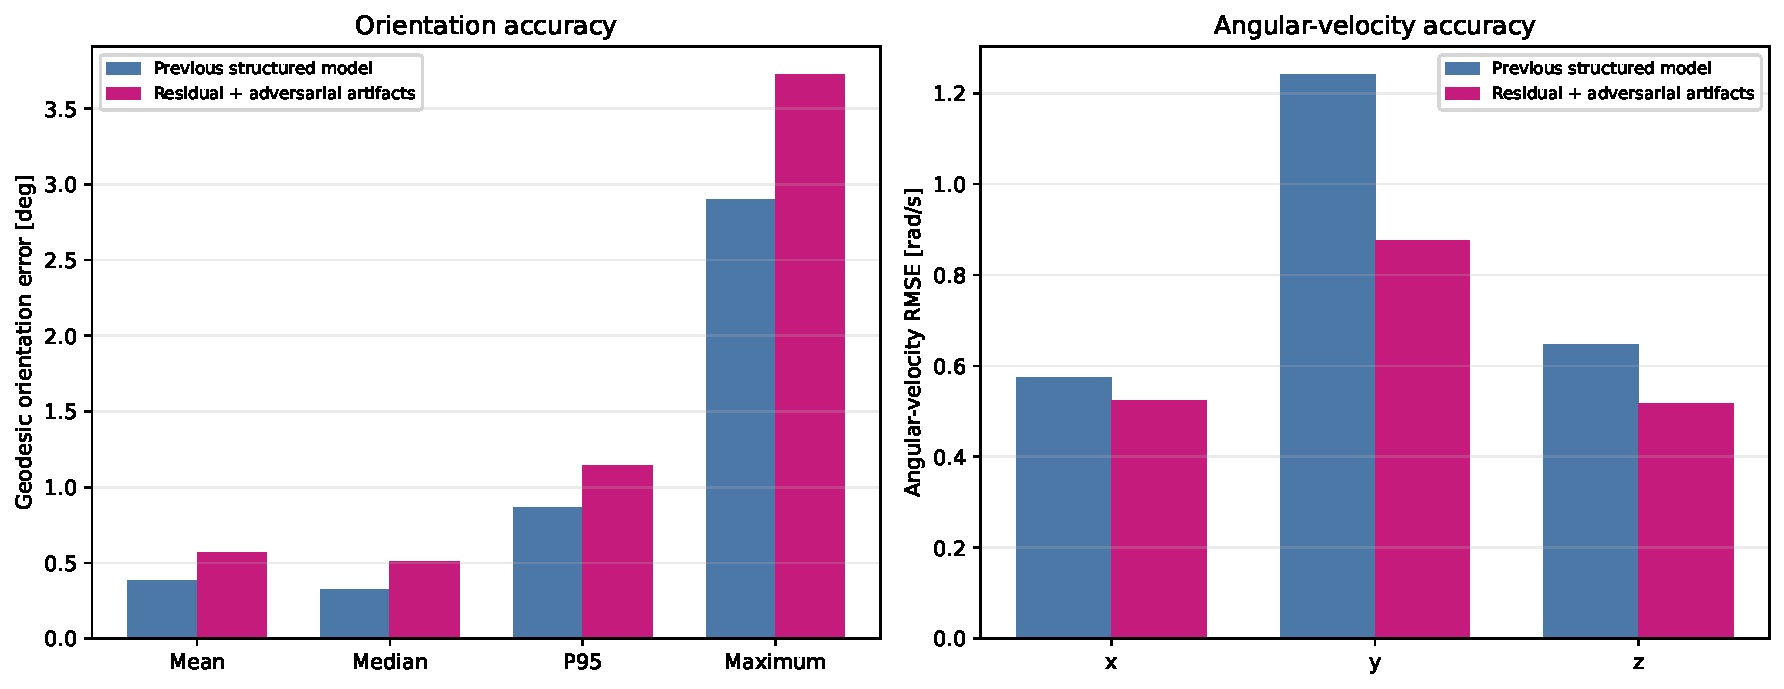
\includegraphics[width=.98\textwidth]{figures/state_comparison.pdf}\caption{State accuracy comparison. Lower is better for every bar.}\end{figure}
\begin{figure}[htbp]\centering
\includegraphics[width=.9\textwidth]{figures/angular_velocity_component_scatter.png}\caption{Current angular-velocity predictions versus ground truth.}\end{figure}

The generator improves on all axes, with the largest gain in $y$. This is compatible with the training design: the physical feature predictor and adversarial competition may force $\xi$ to carry a cleaner motion signal. However, a single run cannot establish causality; different checkpoint epoch and optimisation noise remain alternative explanations.

\section{Temporal intervention results}
The reversed sequence has mean speed $29.179$ rad/s compared with $29.172$ rad/s forward. The reversal residual improves from $1.107$ to $0.918$ rad/s. Repeated frames produce $0.0833$ rad/s, compared with $0.0674$ rad/s previously; both are effectively near zero relative to the 29.17 rad/s forward speed. Shuffling strongly changes the inferred motion.

\begin{figure}[htbp]\centering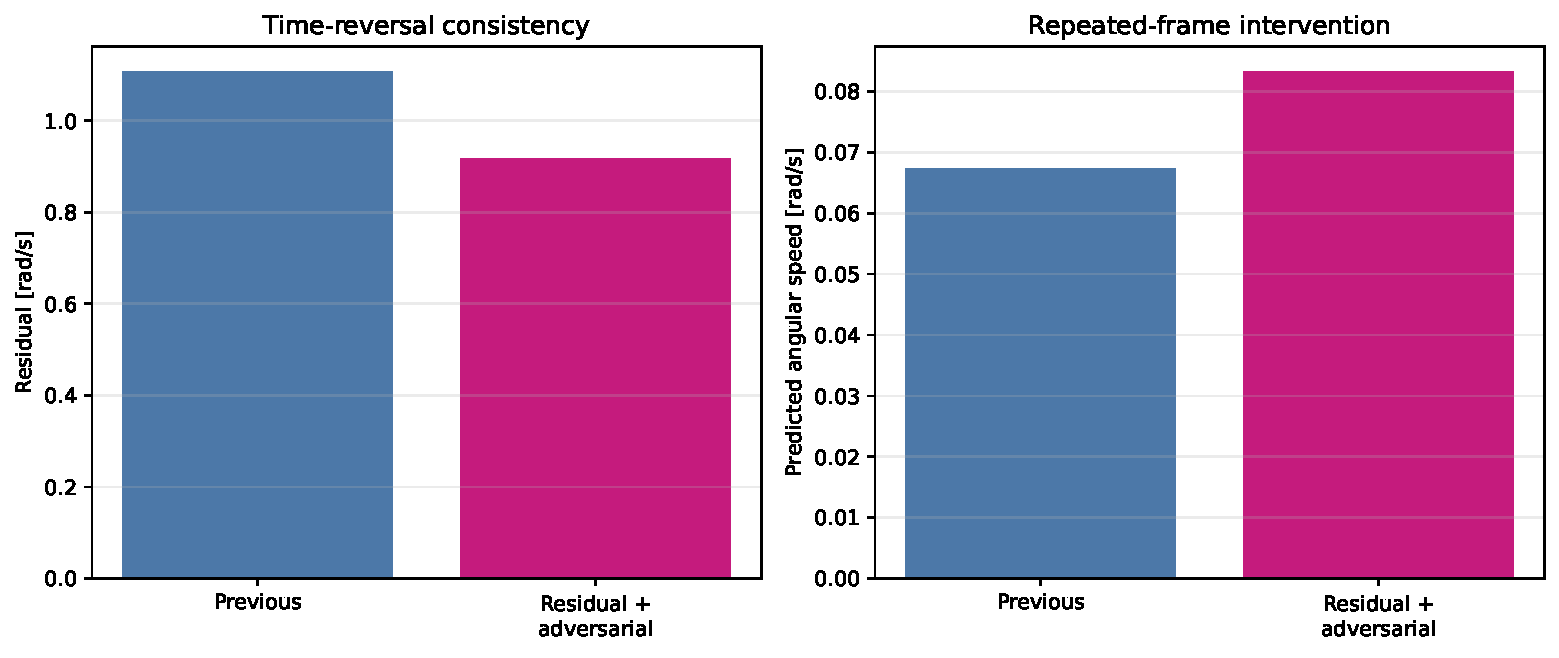
\includegraphics[width=.78\textwidth]{figures/intervention_comparison.pdf}\caption{Temporal intervention comparison. Lower is better.}\end{figure}

These interventions confirm that the canonical generator still responds to directed temporal change and does not infer rotation merely from static appearance.

\section{Intrinsic group geometry}
\subsection{Validity}
Mean orthogonality residual is $1.54\times10^{-7}$ and mean determinant residual is $9.32\times10^{-8}$. These values verify numerical group membership. Since the rotation is constructed through a 6D projection, this result is an implementation validation rather than evidence of learned generalisation.

\subsection{One-step and inverse consistency}
\begin{table}[htbp]\centering\caption{Intrinsic group consistency.}\begin{tabular}{lrrrr}\toprule
Metric & Previous mean & Current mean & Previous P95 & Current P95\\\midrule
One-step [rad] & 0.01247 & 0.01261 & 0.02907 & 0.02840\\
Inverse [rad] & 0.001775 & 0.002523 & 0.003997 & 0.004956\\\bottomrule
\end{tabular}\end{table}
The one-step mean is almost unchanged, while its P95 is slightly better. Inverse consistency becomes worse but remains small: the current mean is $0.145^\circ$.

\subsection{Finite-horizon composition}
At nine intervals, mean rollout error increases from $2.363^\circ$ to $2.466^\circ$, whereas P95 improves from $5.619^\circ$ to $4.957^\circ$. The current model therefore has slightly worse average accumulation but fewer large tail errors.

\begin{figure}[htbp]\centering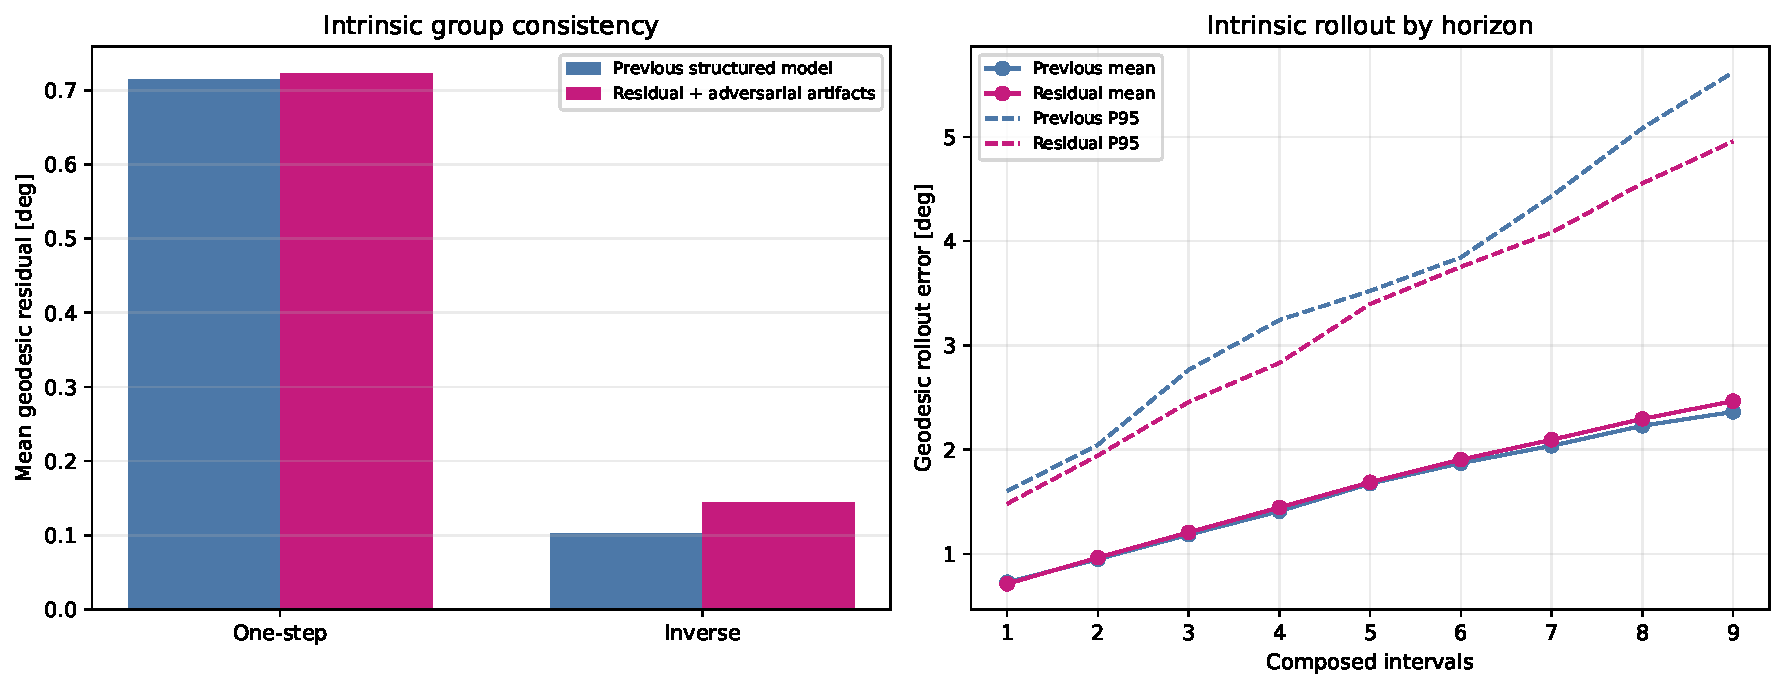
\includegraphics[width=.96\textwidth]{figures/geometry_comparison.pdf}\caption{Intrinsic consistency and recursive rollout.}\end{figure}

The rollout is not autonomous: each interval generator is inferred from both endpoint images. It tests composition of inferred increments, not prediction without future observations.

\section{Did artifact disentanglement improve?}
\subsection{Post-split causal bypass}
The zero-artifact bypass test reports
\begin{equation}
\Delta\omega_{zero\ artifact}=0.0\ \mathrm{rad/s}
\end{equation}
for both mean and P95. This proves that, after sectorisation, the physical angular-velocity output does not causally consume the artifact tensor. This is an architectural isolation test, not an information test.

\subsection{Held-out artifact probe}
\begin{table}[htbp]\centering\caption{Angular velocity decoded from motion artifacts.}\begin{tabular}{lrrrr}\toprule
Axis & Previous $R^2$ & Current $R^2$ & Previous RMSE & Current RMSE\\\midrule
$x$ & 0.99751 & 0.99471 & 0.894 & 1.302\\
$y$ & 0.99592 & 0.99127 & 1.103 & 1.614\\
$z$ & 0.99733 & 0.99185 & 0.903 & 1.580\\\bottomrule
\end{tabular}\end{table}

Mean component $R^2$ decreases from approximately 0.9969 to 0.9926. Leakage is therefore reduced, but only modestly. The artifact remains an excellent linear representation of angular velocity.

\begin{figure}[htbp]\centering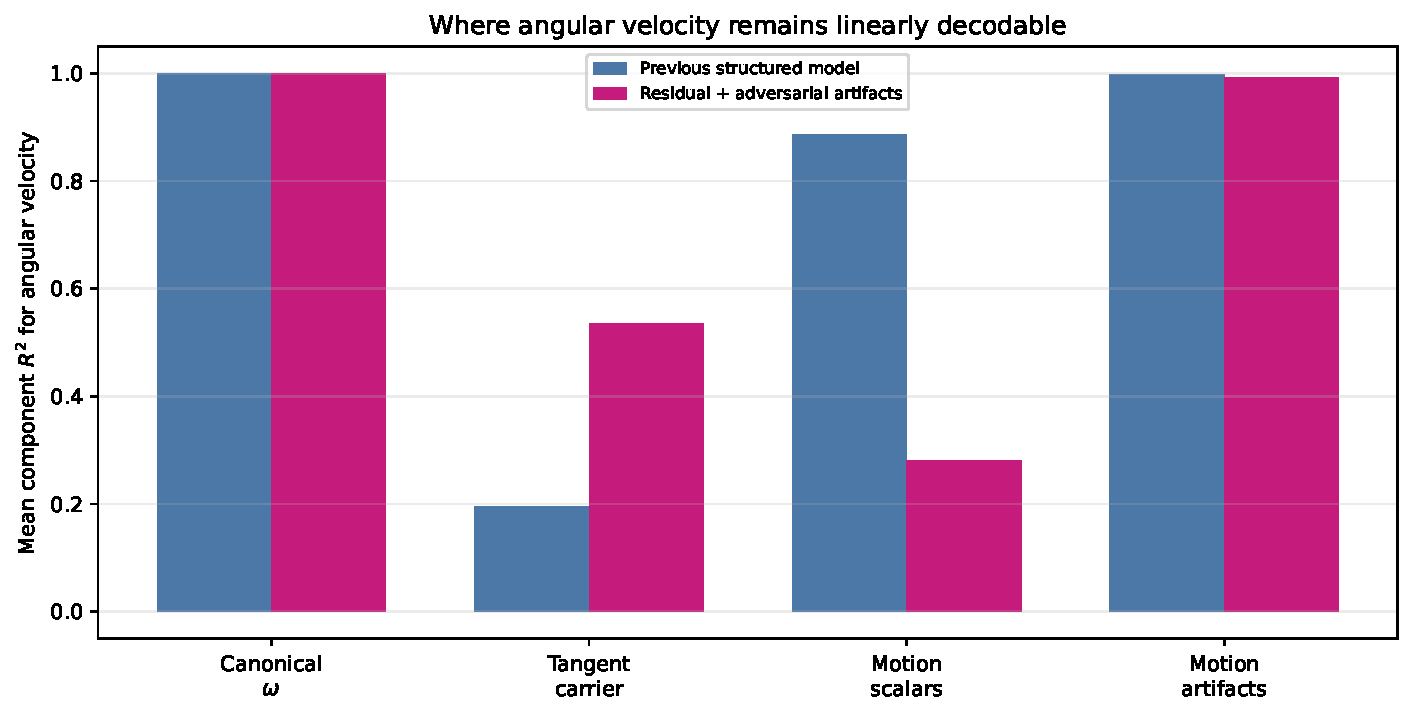
\includegraphics[width=.85\textwidth]{figures/leakage_comparison.pdf}\caption{Sector-wise angular-velocity decodability. The artifact bar remains very high.}\end{figure}

\begin{keyresult}
The artifact treatment does not achieve the primary disentanglement objective. The canonical generator is sufficient and artifact bypass is exact, but the artifact latent still redundantly contains nearly all signed angular-velocity information.
\end{keyresult}

\subsection{Motion scalar sector}
The motion-invariant sector changes more substantially. Mean component $R^2$ decreases from approximately 0.886 to 0.281. The tangent carrier improves from mean $R^2\approx0.195$ to $0.535$. This suggests that representational allocation changed: less signed angular velocity resides in scalar motion features, and more recoverable rotational structure appears in the prescribed tangent carrier.

\subsection{Effective rank}
\begin{figure}[htbp]\centering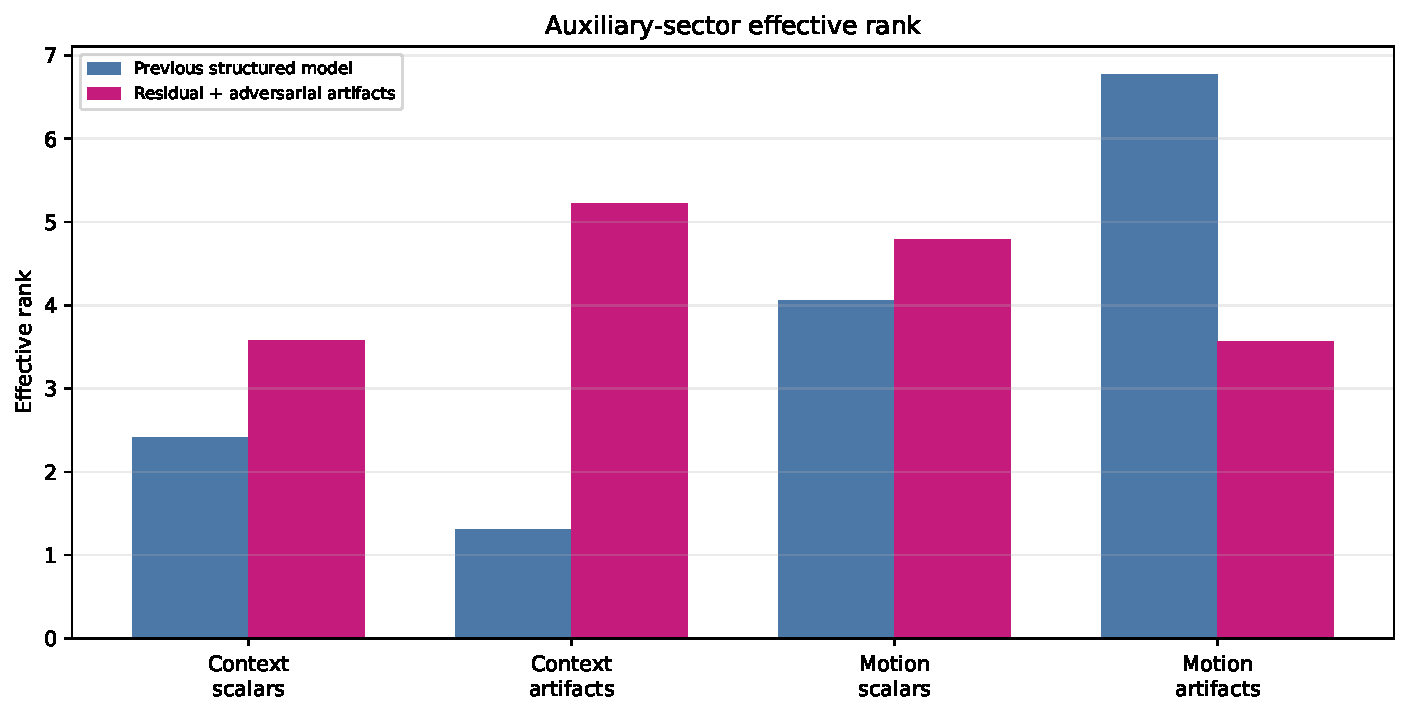
\includegraphics[width=.87\textwidth]{figures/rank_comparison.pdf}\caption{Effective ranks of auxiliary sectors.}\end{figure}

Context artifacts increase in rank from 1.30 to 5.22, while motion artifacts decrease from 6.77 to 3.56. Context invariants increase from 2.41 to 3.58 and motion invariants from 4.05 to 4.79. The residual objective activates context artifacts more broadly and compresses motion artifacts, but compression alone does not remove their angular-velocity content.

\subsection{Residual utility}
Residual feature reconstruction MSE is reported as 1.034 with P95 1.756. This confirms that the evaluation pipeline measures the positive artifact task. However, no zero-artifact or mean-predictor residual baseline is included, so the absolute value cannot establish that artifacts reconstruct residual observations better than a trivial predictor.

\section{Why the adversarial objective only partly worked}
Several mechanisms plausibly explain the persistent leakage.

\subsection{The residual remains state correlated}
Even a perfect visual residual can depend on rotation. Occlusion, shadows, marker visibility, and projection effects are caused by the same motion. Therefore
\begin{equation}
I(r_t;\omega_t)>0
\end{equation}
can hold even when the structured physical prediction is useful. Asking $\nu_t$ to reconstruct $r_t$ and simultaneously forget $\omega_t$ creates competing objectives.

\subsection{The physics-conditioned predictor is learned, not exact}
$D_p(F_t,G_t,\xi_t,\Delta t)$ is not a geometric renderer or exact feature warp. Any component of rigid motion it fails to explain remains in $r_t$, making physical leakage useful to the residual encoder.

\subsection{Adversarial removal is probe dependent}
A training adversary removes information accessible to that adversary under the selected weight and optimisation schedule. A held-out ridge probe still recovers angular velocity. This indicates the adversarial force was too weak, the reconstruction force too strong, or the residual itself retained a highly linear physical component.

\subsection{The data do not independently vary artifacts}
The controlled dataset has fixed camera, background, markers, and rendering conditions. It contains little evidence that defines an artifact factor independently of physical rotation. Without crossed appearance variation, the separation is statistically underidentified.

\section{Research interpretation}
\begin{verdict}
The current experiment improves the physical generator and changes latent allocation without achieving genuine artifact-motion disentanglement. It establishes causal isolation of the output pathway, not informational independence of the artifact representation.
\end{verdict}

The most defensible claims are:
\begin{enumerate}
\item The structured $SO(3)/\so(3)$ pathway remains valid and accurate after adding residual and adversarial artifact training.
\item Generator RMSE improves on all axes, reversal improves, and rollout tail error improves.
\item Orientation accuracy worsens and inverse consistency becomes less accurate.
\item Zeroing artifacts after the split has no effect on physical output, confirming the intended routing.
\item Artifact angular-velocity leakage decreases slightly but remains extremely high.
\item The scalar motion sector is substantially cleaner, and the tangent carrier becomes more informative.
\end{enumerate}

\section{Recommended next experiments}
\subsection{Measure residual reconstruction against baselines}
Compare $D_\nu(\nu_t)$ against zero, temporal mean, and physics-only predictions. Report normalised explained variance per feature channel rather than raw MSE alone.

\subsection{Increase adversarial strength carefully}
Run a sweep over maximum gradient-reversal strength and cross-covariance weight. Plot a Pareto frontier between artifact leakage and residual reconstruction. A successful setting should reduce held-out $R^2$ without materially harming $\xi$, one-step consistency, or residual reconstruction.

\subsection{Adversary capacity and alternating optimisation}
Train a linear and nonlinear adversary and evaluate with stronger probes not used during training. Alternating adversary and encoder updates may prevent the encoder from exploiting a temporarily weak adversary.

\subsection{Make the physical predictor more geometric}
Rather than learning all of $D_p$, use $G_t$ and $\xi_t$ to warp feature samples or marker-centred features. The artifact residual should be calculated after a physically prescribed transformation whenever possible.

\subsection{Introduce crossed appearance variation}
Render identical physical trajectories under multiple cameras, backgrounds, lighting directions, blur levels, and marker appearances. Require the physical sectors to agree across appearances and the artifact sector to distinguish them. This is the most important data-level improvement.

\subsection{Conditional rather than unconditional separation}
Shadows and visibility are physically caused but non-geometric. A strict independence objective may remove precisely the effects artifacts should represent. Future work should define artifacts conditionally as observation information remaining after physical state and renderer conditions are specified.

\subsection{No-artifact and training-only-artifact ablations}
Compare the current model with a model containing no artifact branch and a model whose artifact head is used only as an auxiliary training objective. These ablations determine whether artifacts help the shared encoder or merely duplicate the physical state.

\section{Representative trajectories}
\begin{figure}[p]\centering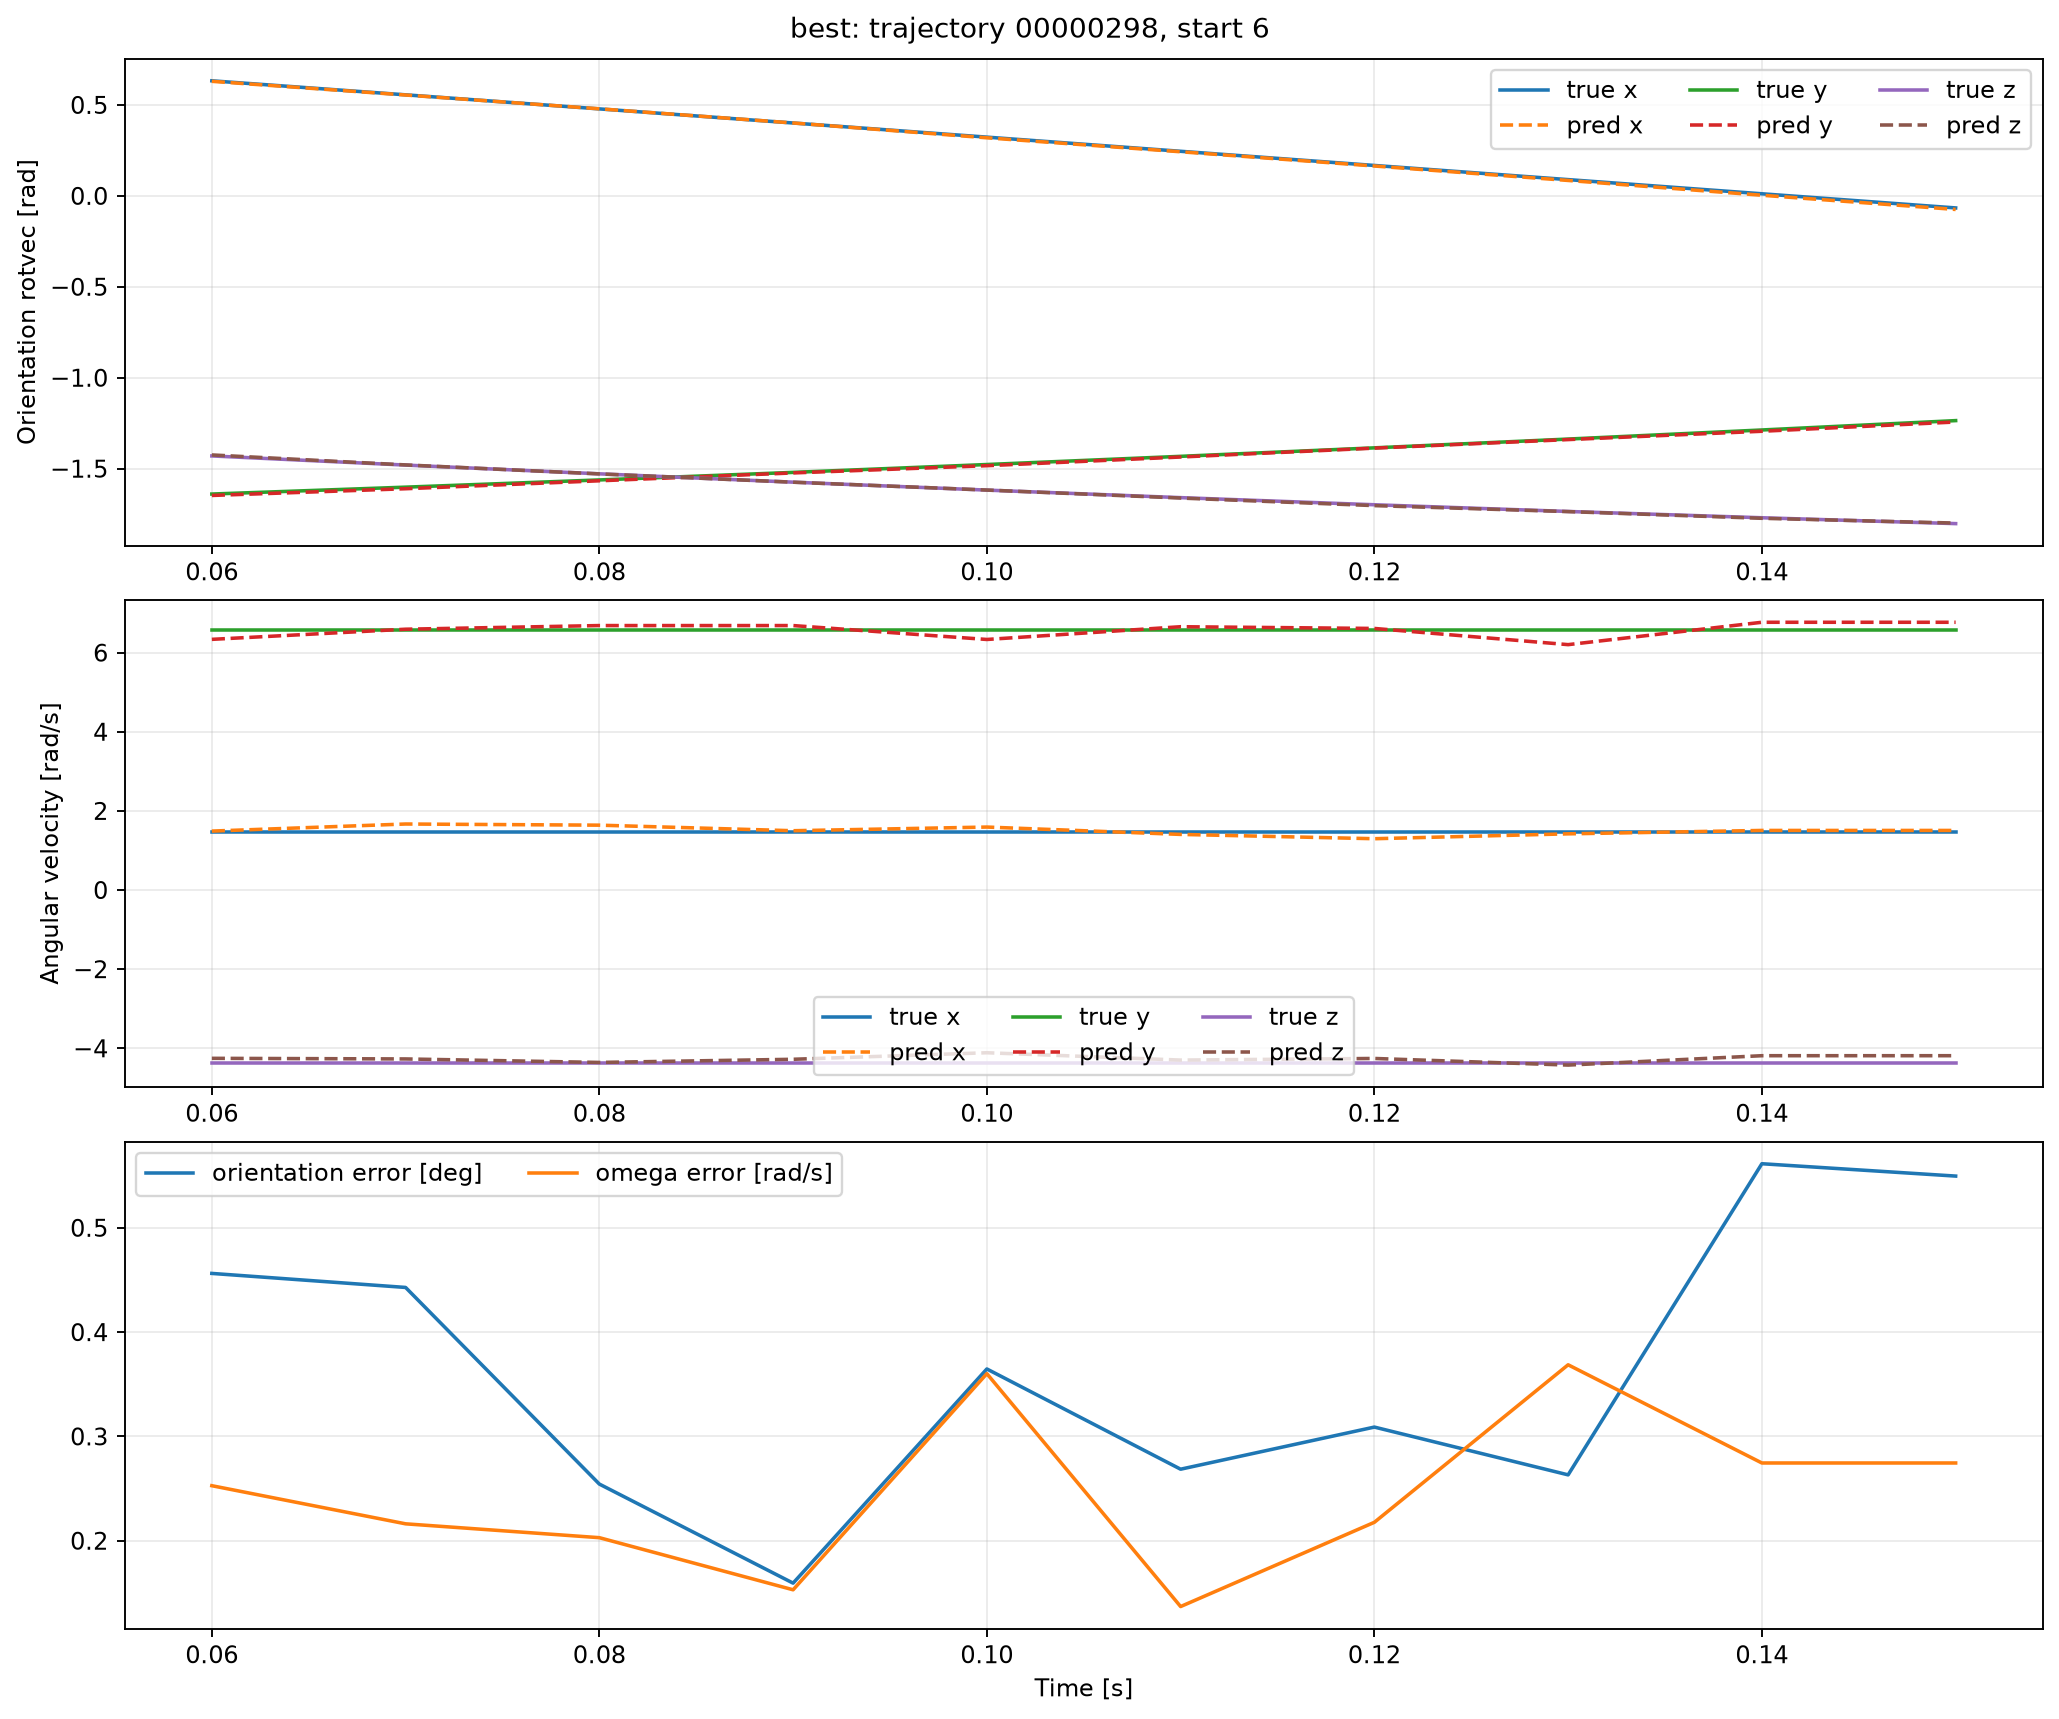
\includegraphics[width=.94\textwidth]{figures/best_00000298_000006.png}\caption{Best evaluated context window.}\end{figure}
\begin{figure}[p]\centering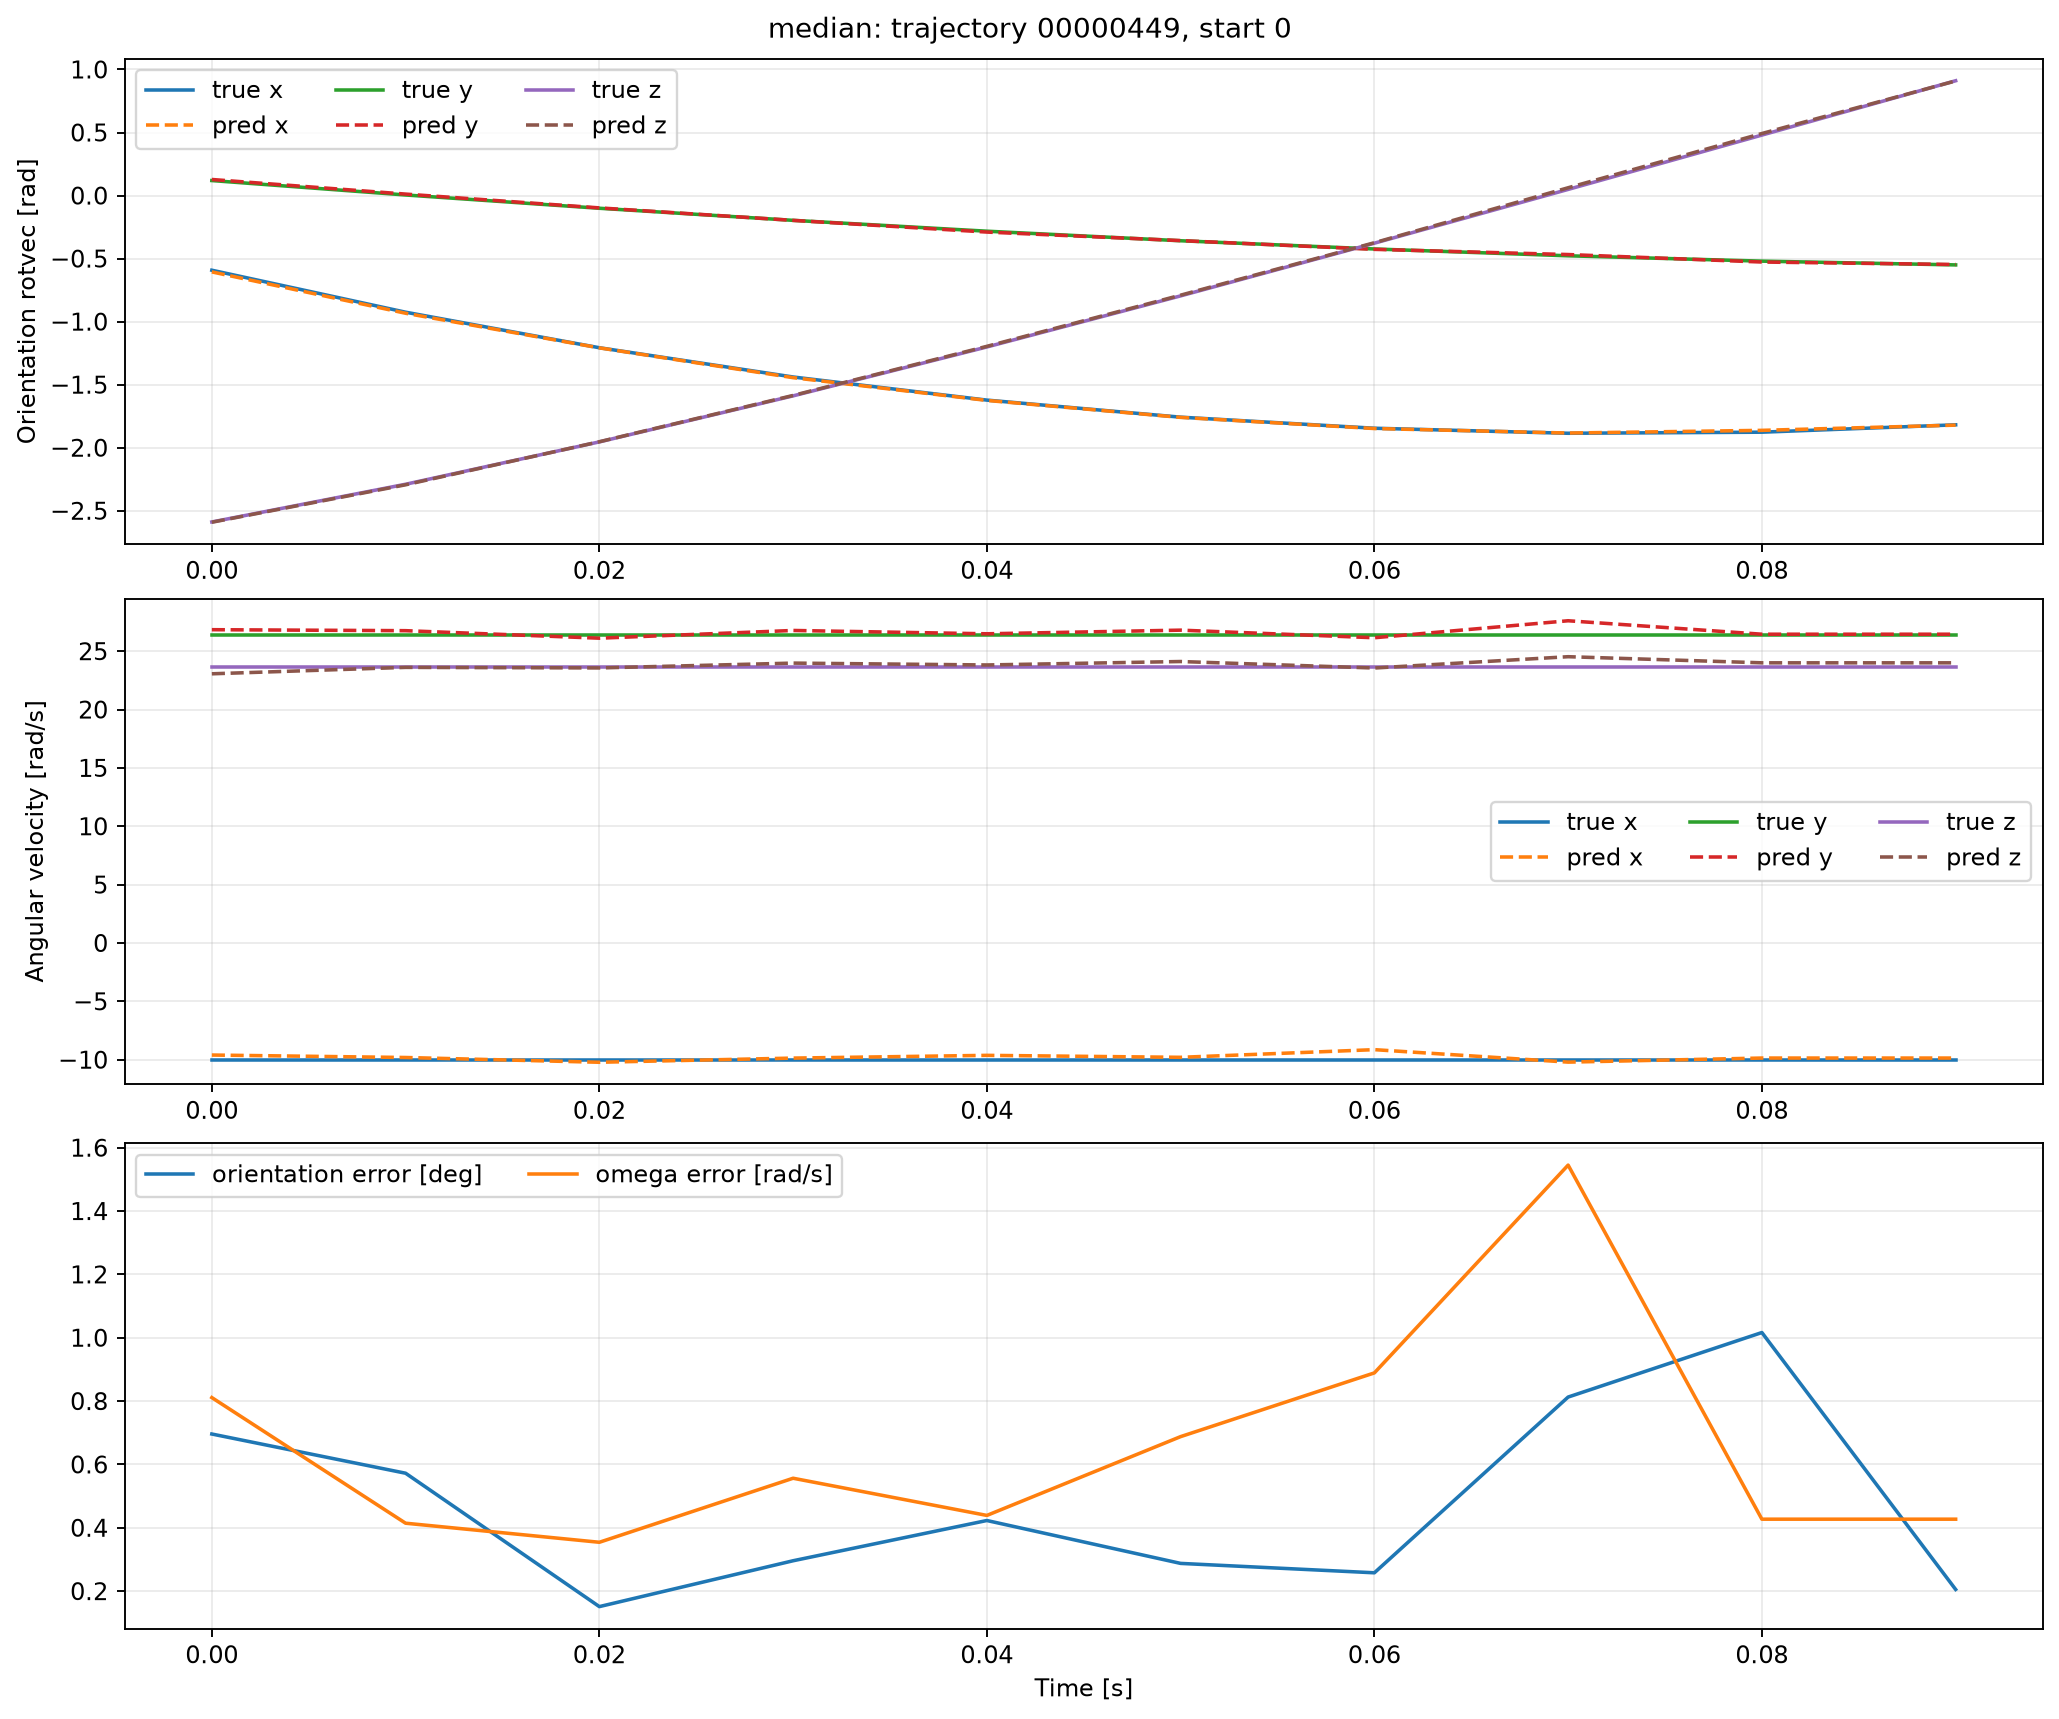
\includegraphics[width=.94\textwidth]{figures/median_00000449_000000.png}\caption{Median evaluated context window.}\end{figure}
\begin{figure}[p]\centering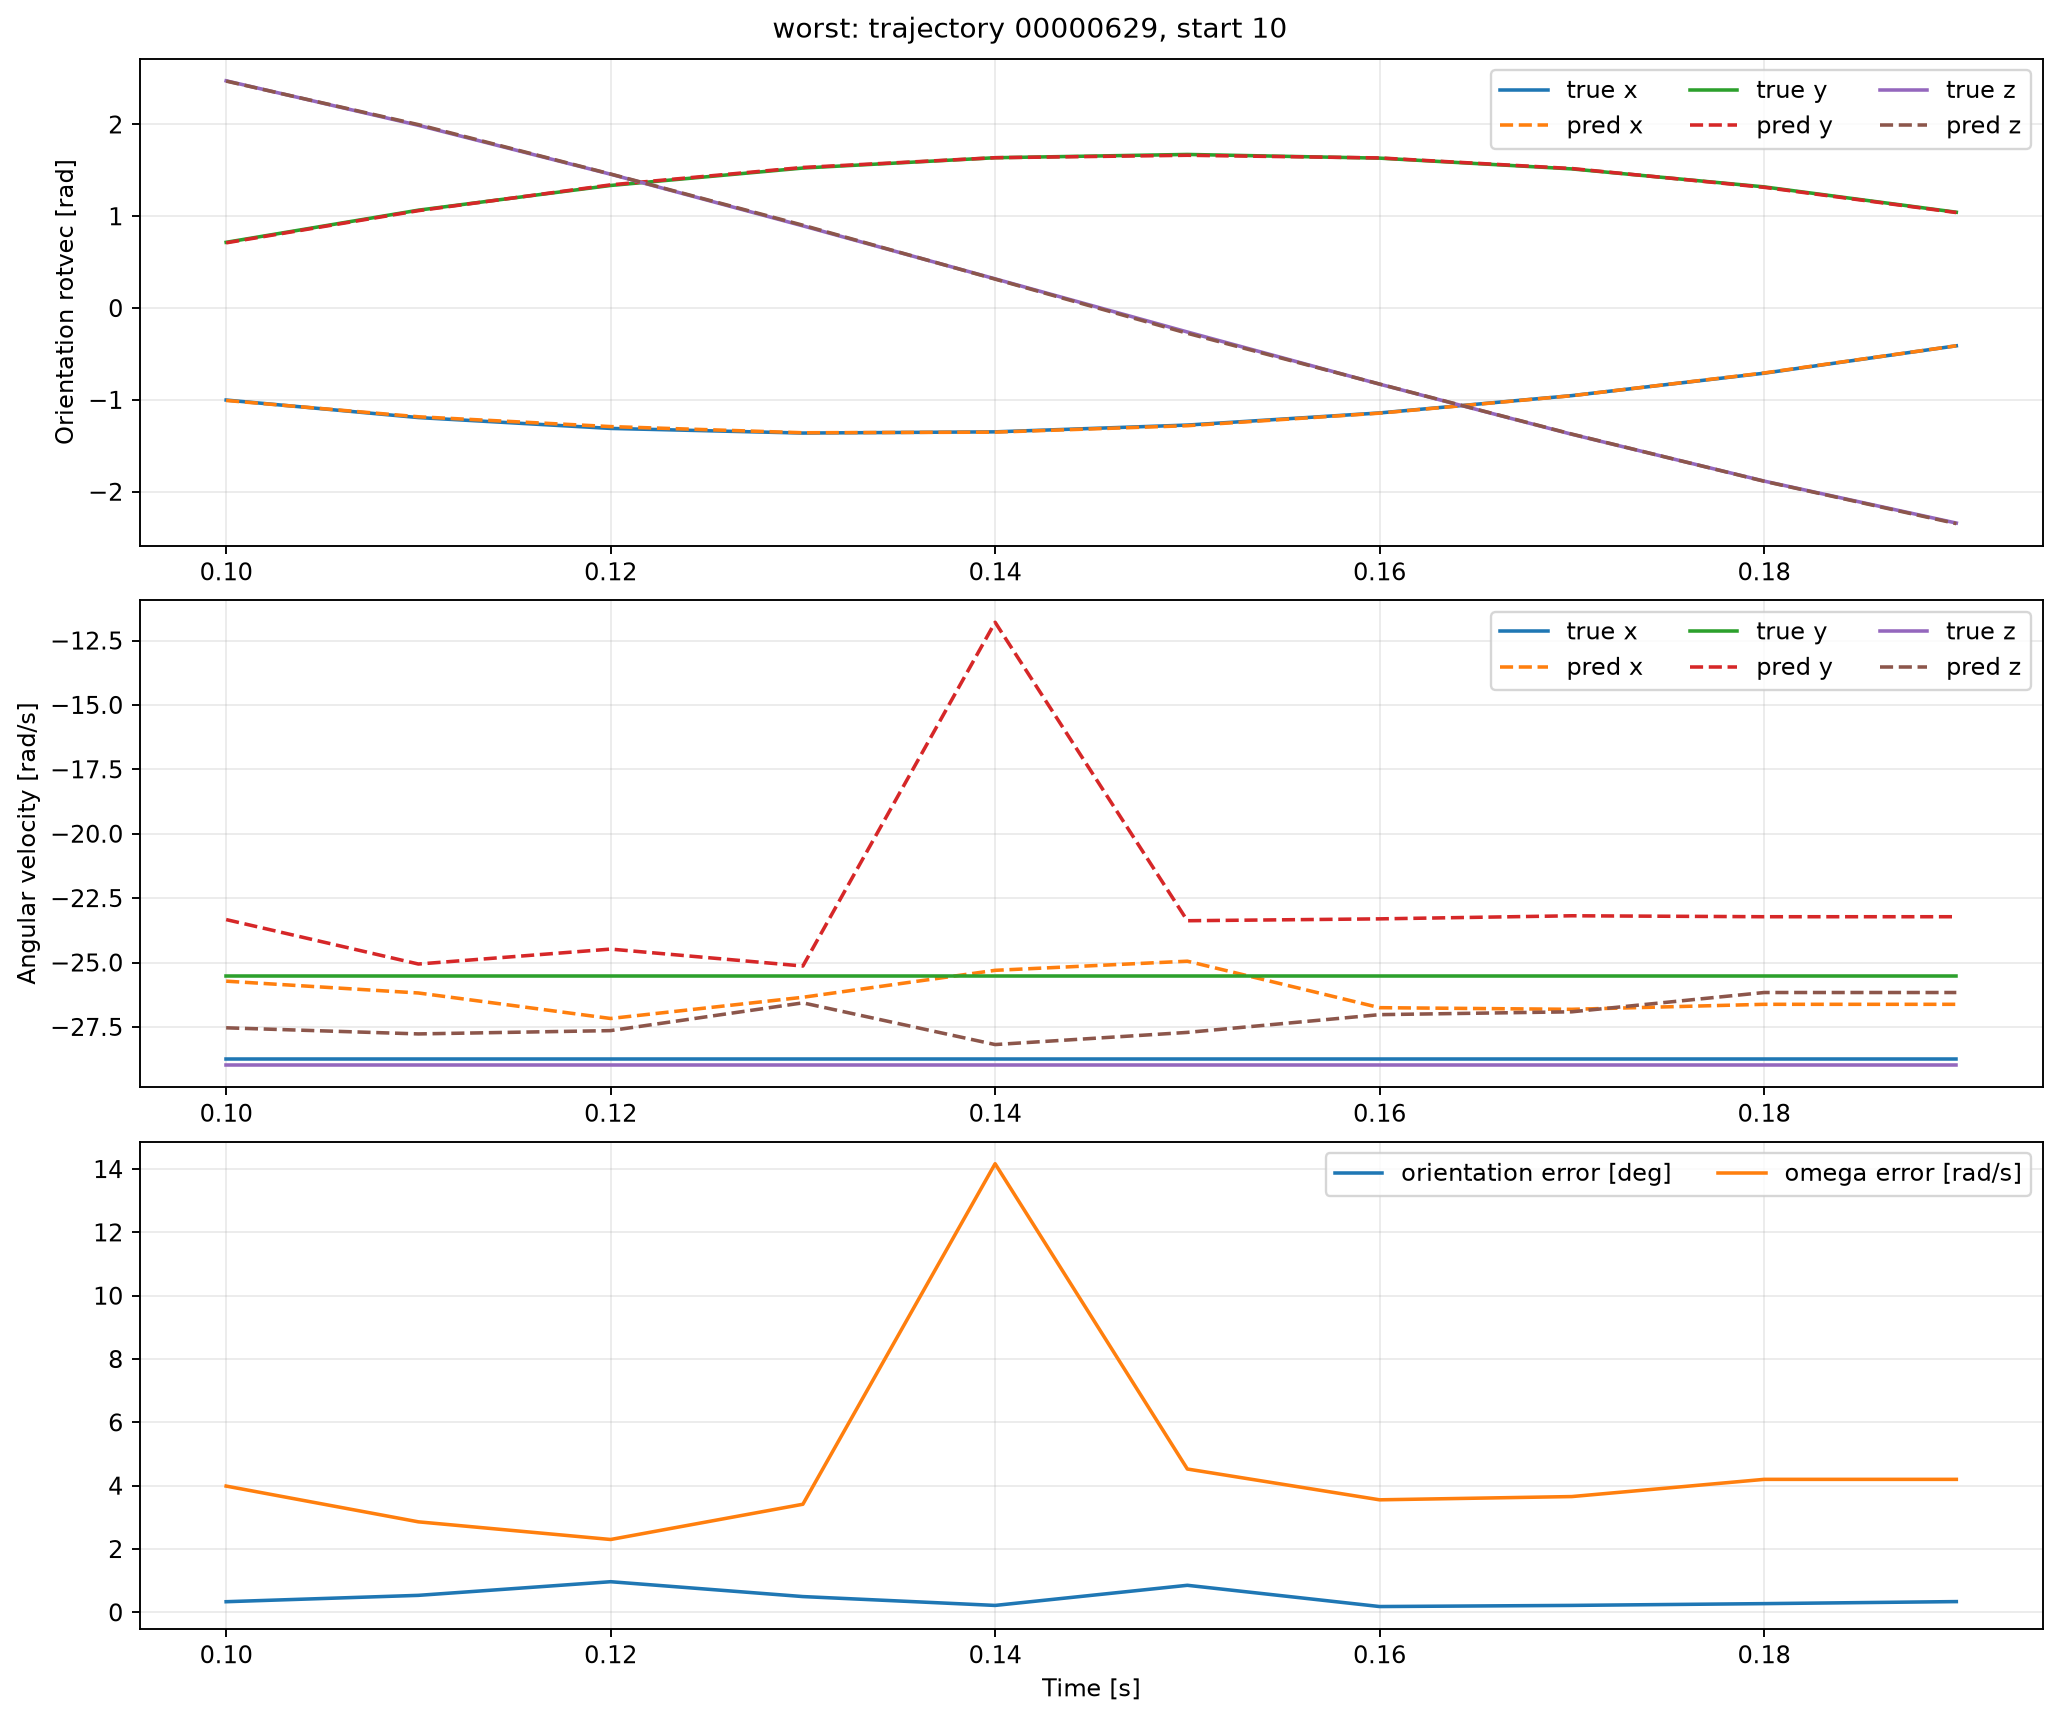
\includegraphics[width=.94\textwidth]{figures/worst_00000629_000010.png}\caption{Worst selected context window.}\end{figure}\clearpage

\section{Conclusion}
The physics-residual artifact strategy is mathematically better motivated than a generic parallel artifact head. It gives artifacts a positive observational role, blocks their direct use by physical output, and introduces explicit pressure against rotational leakage. The experiment preserves excellent state estimation and improves canonical angular-velocity accuracy. It also confirms that artifact bypass is exact.

The central disentanglement result is nevertheless negative or, at best, preliminary. Motion artifacts still predict angular velocity with mean $R^2$ above 0.99. The improvement from the previous model is too small to claim that artifacts now represent predominantly nonphysical image variation. The strongest progress is seen in the motion scalar sector and tangent carrier, not in artifact independence.

This result is scientifically useful. It demonstrates that naming sectors, subtracting a learned physical prediction, and adding weak adversaries are not sufficient when physical motion remains statistically entangled with residual visual effects. Stronger geometric residualisation, better adversarial evaluation, and independently varied appearance data are required. The structured physical pathway remains a sound foundation; the remaining challenge is to make auxiliary observation representations complement it rather than replicate it.

\appendix
\section{Numerical summary}
\begin{itemize}
\item Orientation mean/median/P95/max: 0.5657/0.5121/1.1407/3.7239 degrees.
\item Angular-velocity RMSE: 0.5236, 0.8765, 0.5173 rad/s.
\item Reversal residual: 0.9178 rad/s; repeated-frame speed: 0.0833 rad/s.
\item One-step group residual: 0.01261 rad mean; inverse residual: 0.002523 rad mean.
\item Nine-interval rollout: 2.466 degrees mean and 4.957 degrees P95.
\item Artifact probe $R^2$: 0.9947, 0.9913, 0.9919.
\item Zero-artifact angular-velocity delta: exactly 0.0 rad/s in the reported evaluation.
\item Residual reconstruction MSE: 1.034 mean, 1.756 P95.
\end{itemize}

\section{Reproducibility checklist}
\begin{itemize}
\item Preserve trajectory-disjoint splits and identical evaluation windows across comparisons.
\item Save exact effective training configuration and checkpoint epoch.
\item Report adversary strength schedule and all artifact objective weights.
\item Evaluate with probes stronger than those used adversarially during training.
\item Include trivial residual-reconstruction baselines.
\item Run several random seeds before attributing metric changes to architecture.
\item Keep decoded-state refinement disabled while evaluating latent geometry.
\end{itemize}

\bibliographystyle{plainnat}\bibliography{references}
\end{document}
